\begin{frame}{Αυτόνομη πλοήγηση: Συστατικά}

\definecolor{r}{RGB}{255 0 0}
\definecolor{rr}{RGB}{168 0 0}
\definecolor{g}{RGB}{0 255 0}
\definecolor{gg}{RGB}{67 120 17}
\definecolor{gr}{RGB}{128 128 128}
\definecolor{b}{RGB}{22 38 252}

\noindent\makebox[\linewidth][c]{%
\begin{minipage}{\linewidth}
  \begin{minipage}{0.4\linewidth}
    \begin{figure}
      

\tikzset{every picture/.style={line width=0.75pt}} %set default line width to 0.75pt

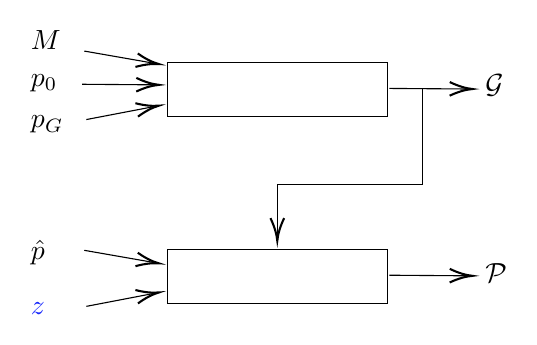
\begin{tikzpicture}[x=0.75pt,y=0.75pt,yscale=-1,xscale=1]
%uncomment if require: \path (0,300); %set diagram left start at 0, and has height of 300

%Shape: Rectangle [id:dp731904440257259]
\draw   (100,131.14) -- (206,131.14) -- (206,157.14) -- (100,157.14) -- cycle ;
%Straight Lines [id:da2806201022146415]
\draw    (60,125.71) -- (94.03,131.66) ;
\draw [shift={(96,132)}, rotate = 189.9] [color={rgb, 255:red, 0; green, 0; blue, 0 }  ][line width=0.75]    (10.93,-3.29) .. controls (6.95,-1.4) and (3.31,-0.3) .. (0,0) .. controls (3.31,0.3) and (6.95,1.4) .. (10.93,3.29)   ;
%Straight Lines [id:da6687229108601818]
\draw    (59,141.71) -- (94,141.98) ;
\draw [shift={(96,142)}, rotate = 180.44] [color={rgb, 255:red, 0; green, 0; blue, 0 }  ][line width=0.75]    (10.93,-3.29) .. controls (6.95,-1.4) and (3.31,-0.3) .. (0,0) .. controls (3.31,0.3) and (6.95,1.4) .. (10.93,3.29)   ;
%Straight Lines [id:da6113858760433817]
\draw    (61,158.71) -- (94.04,152.38) ;
\draw [shift={(96,152)}, rotate = 169.14] [color={rgb, 255:red, 0; green, 0; blue, 0 }  ][line width=0.75]    (10.93,-3.29) .. controls (6.95,-1.4) and (3.31,-0.3) .. (0,0) .. controls (3.31,0.3) and (6.95,1.4) .. (10.93,3.29)   ;
%Straight Lines [id:da8568820791470133]
\draw    (207,143.71) -- (245,143.99) ;
\draw [shift={(247,144)}, rotate = 180.41] [color={rgb, 255:red, 0; green, 0; blue, 0 }  ][line width=0.75]    (10.93,-3.29) .. controls (6.95,-1.4) and (3.31,-0.3) .. (0,0) .. controls (3.31,0.3) and (6.95,1.4) .. (10.93,3.29)   ;
%Shape: Rectangle [id:dp7904387701938098]
\draw   (100,221.14) -- (206,221.14) -- (206,247.14) -- (100,247.14) -- cycle ;
%Straight Lines [id:da685491548836421]
\draw    (153,190) -- (153,215.14) ;
\draw [shift={(153,217.14)}, rotate = 270] [color={rgb, 255:red, 0; green, 0; blue, 0 }  ][line width=0.75]    (10.93,-3.29) .. controls (6.95,-1.4) and (3.31,-0.3) .. (0,0) .. controls (3.31,0.3) and (6.95,1.4) .. (10.93,3.29)   ;
%Straight Lines [id:da5097874694401365]
\draw    (61,248.71) -- (94.04,242.38) ;
\draw [shift={(96,242)}, rotate = 169.14] [color={rgb, 255:red, 0; green, 0; blue, 0 }  ][line width=0.75]    (10.93,-3.29) .. controls (6.95,-1.4) and (3.31,-0.3) .. (0,0) .. controls (3.31,0.3) and (6.95,1.4) .. (10.93,3.29)   ;
%Straight Lines [id:da08555513808334525]
\draw    (207,233.71) -- (245,233.99) ;
\draw [shift={(247,234)}, rotate = 180.41] [color={rgb, 255:red, 0; green, 0; blue, 0 }  ][line width=0.75]    (10.93,-3.29) .. controls (6.95,-1.4) and (3.31,-0.3) .. (0,0) .. controls (3.31,0.3) and (6.95,1.4) .. (10.93,3.29)   ;
%Straight Lines [id:da37777604435779377]
\draw    (153,190) -- (223,190) ;
%Straight Lines [id:da9672472931226035]
\draw    (223,144) -- (223,190) ;
%Straight Lines [id:da7265677070785583]
\draw    (60,221.71) -- (94.03,227.66) ;
\draw [shift={(96,228)}, rotate = 189.9] [color={rgb, 255:red, 0; green, 0; blue, 0 }  ][line width=0.75]    (10.93,-3.29) .. controls (6.95,-1.4) and (3.31,-0.3) .. (0,0) .. controls (3.31,0.3) and (6.95,1.4) .. (10.93,3.29)   ;

% Text Node
\draw (103,137) node [anchor=north west][inner sep=0.75pt]   [align=left] {};
% Text Node
\draw (33,114.71) node [anchor=north west][inner sep=0.75pt]   [align=left] {$\bm{M}$};
% Text Node
\draw (33,135.71) node [anchor=north west][inner sep=0.75pt]   [align=left] {$\bm{p}_0$};
% Text Node
\draw (33,155.71) node [anchor=north west][inner sep=0.75pt]   [align=left] {$\bm{p}_G$};
% Text Node
\draw (252,135.71) node [anchor=north west][inner sep=0.75pt]   [align=left] {$\mathcal{G}$};
% Text Node
\draw (106,228) node [anchor=north west][inner sep=0.75pt]   [align=left] {};
% Text Node
\draw (33,215.71) node [anchor=north west][inner sep=0.75pt]   [align=left] {$\hat{\bm{p}}$};
% Text Node
\draw (33,245.71) node [anchor=north west][inner sep=0.75pt]   [align=left] {\textcolor{b}{$\bm{z}$}};
% Text Node
\draw (252,227) node [anchor=north west][inner sep=0.75pt]   [align=left] {$\mathcal{P}$};


\end{tikzpicture}


    \end{figure}
  \end{minipage}
  \hfill
  \begin{minipage}{0.5\linewidth}
    \begin{figure}
      \includegraphics[height=120pt,width=213.3pt]{./figures/slides/ch3/relief_video_1_imgs/relief_video_1_109}
      \begin{textblock}{4}(12.3,7.2)
        \scriptsize $\textcolor{rr}{\mathcal{G}}$
      \end{textblock}
      \begin{textblock}{4}(9.1,6.0)
        \scriptsize $\textcolor{gg}{\mathcal{P}}$
      \end{textblock}
    \end{figure}
  \end{minipage}
\end{minipage}
}

\note{\footnotesize
Δεδομένων αυτών η αυτόνομη πλοήγηση συνίσταται σε δύο μέρη: \\
αφενός χρειάζεται ένας αλγόριθμος που δέχεται τον χάρτη, και την αρχική και τελική στάση \\
και παράγει ένα μονοπάτι το οποίο συνδέει την αρχική με την τελική στάση χωρίς να
τέμνει εμπόδια του χάρτη, \\
και αφετέρου ένας ελεγκτής κίνησης, ο οποίος, δεδομένου του μονοπατιού, της
στιγμιαίας εκτίμησης για τη στάση του ρομπότ, και μετρήσεις από αισθητήρες
παράγει εντολές κίνησης τις οποίες λαμβάνουν ως είσοδο οι κινητήρες του
ρομπότ ώστε αυτό να κινείται πάνω στο μονοπάτι που παρήγαγε ο πρώτος
αλγόριθμος}

\end{frame}
